\chapter{Resultados e Discussão}

Este capítulo apresenta os resultados obtidos durante o desenvolvimento e a avaliação da proposta de solução BURI. O conteúdo encontra-se 
organizado da seguinte forma: primeiramente, aborda-se a análise das respostas de dois questionários aplicados aos alunos sobre o sistema 
de monitoramento na Seção \ref{questionario}. O primeiro questionário foi aplicado na fase de especificação, enquanto o segundo, na etapa de teste de usabilidade. 
Em seguida, realiza-se a avaliação do sistema de alerta na Seção \ref{alerta}, cujas funcionalidades não foram abordadas na etapa anterior. Por fim, apresenta-se na Seção \ref{comparacao} uma análise comparativa 
entre a solução proposta neste trabalho de conclusão de curso e trabalhos acadêmicos de referência.

\section{Análise dos questionários}\label{questionario}

Sobre o primeiro questionário, a primeira pergunta analisada é sobre o preço justo de um dispositivo de medição da qualidade do ar. Do total de 58 entrevistados, 48,3\% 
aceitariam gastar o valor de R\$ 200 até, no máximo, R\$ 500 reais com o protótipo embarcado. Esse dado é um fator positivo do projeto BURI, pois o custo final de montagem do 
protótipo é inferior ao custo da expectativa dos potenciais usuários, totalizando R\$ 146,25 segundo os dados obtidos da Tabela \ref{tabPrecoHardware}.

\begin{figure}[ht]
    \centering
    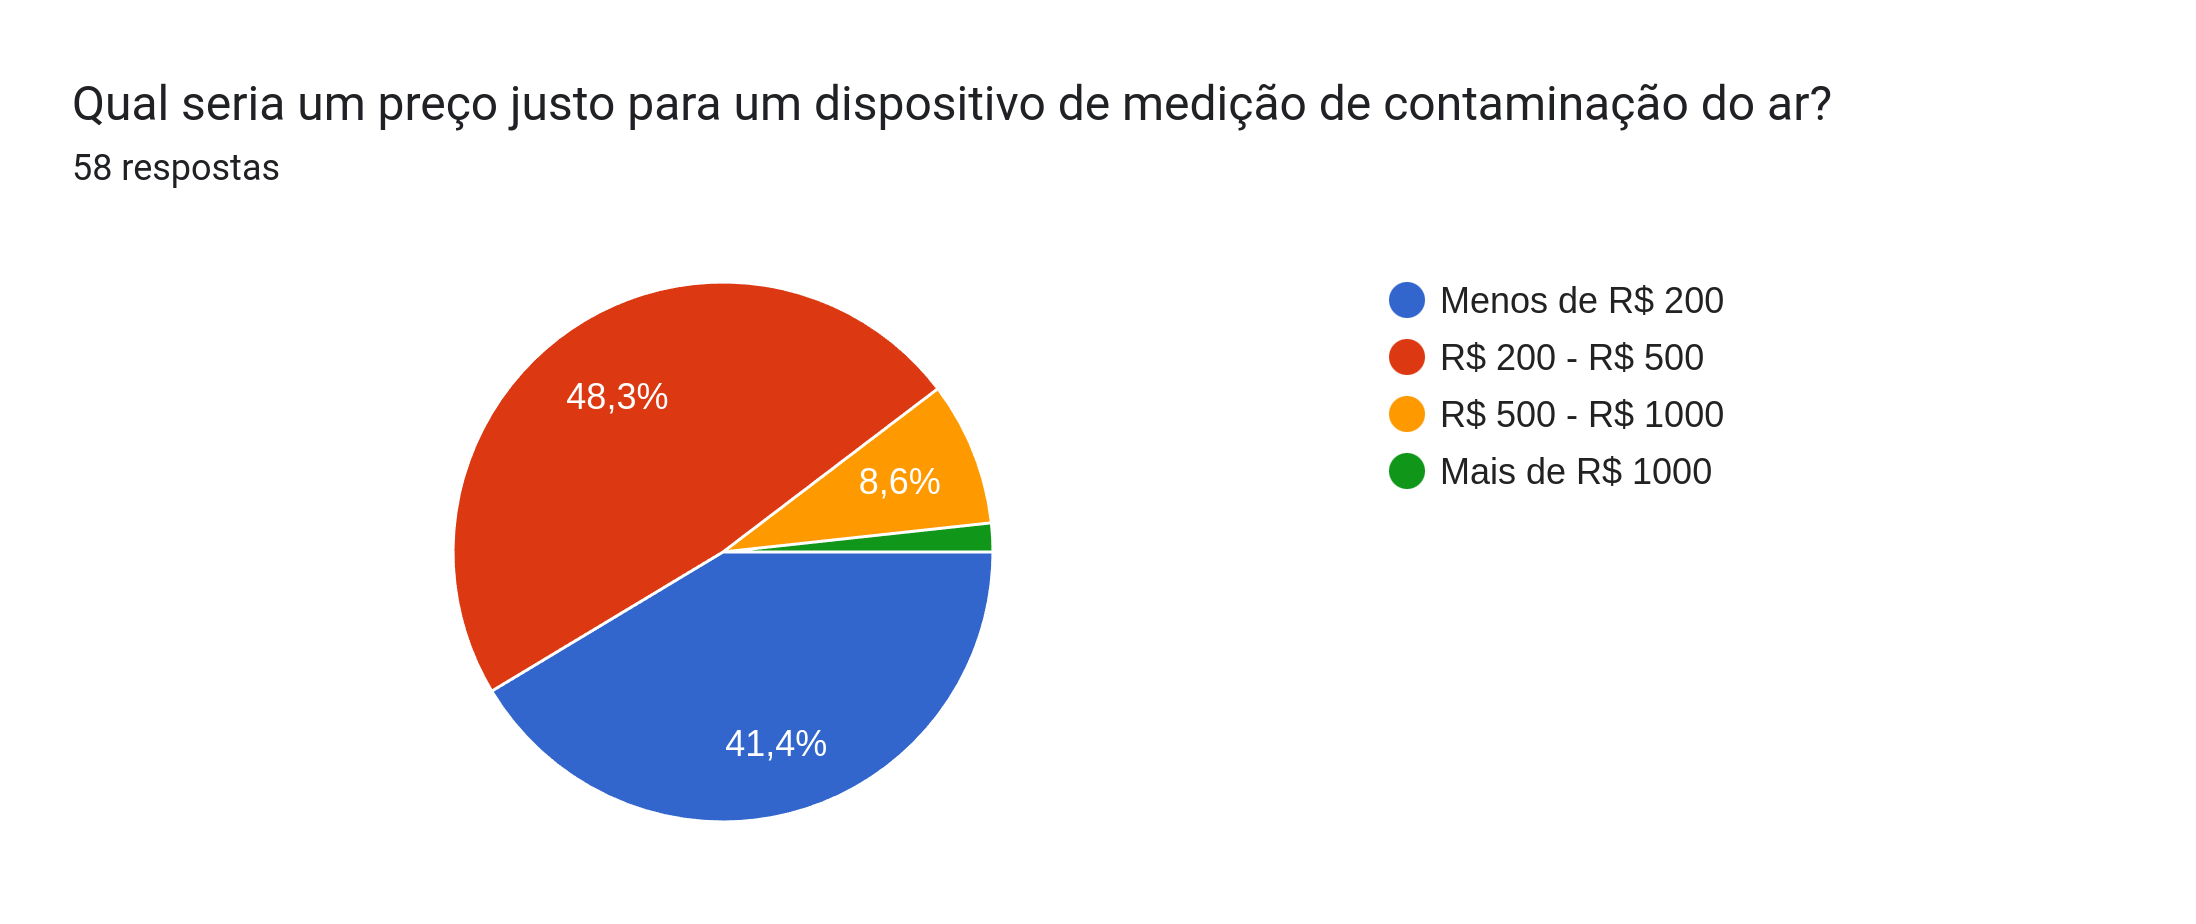
\includegraphics[width=.64\textwidth]{img/questionario/1/graf-preco-hardware.png}
    \caption{Resultado do questionamento sobre o preço justo do dispositivo embarcado de monitoramento da qualidade do ar. Fonte: Autor.}\label{grafPrecoJusto}
\end{figure}

Quanto à frequência de obtenção de dados, a maioria dos usuários optou por receber informações diariamente. No entanto, o dispositivo embarcado realiza a coleta e o envio de dados ao servidor a cada minuto, uma vez 
que o monitoramento da concentração de monóxido de carbono exige intervalos de coleta curtos devido à gravidade progressiva dos efeitos da intoxicação no organismo. Além disso, o sistema também intervém em situações 
de problemas ambientais, notificando o usuário por meio do aplicativo sobre eventos de risco à saùde.
\begin{figure}[ht]
    \centering
    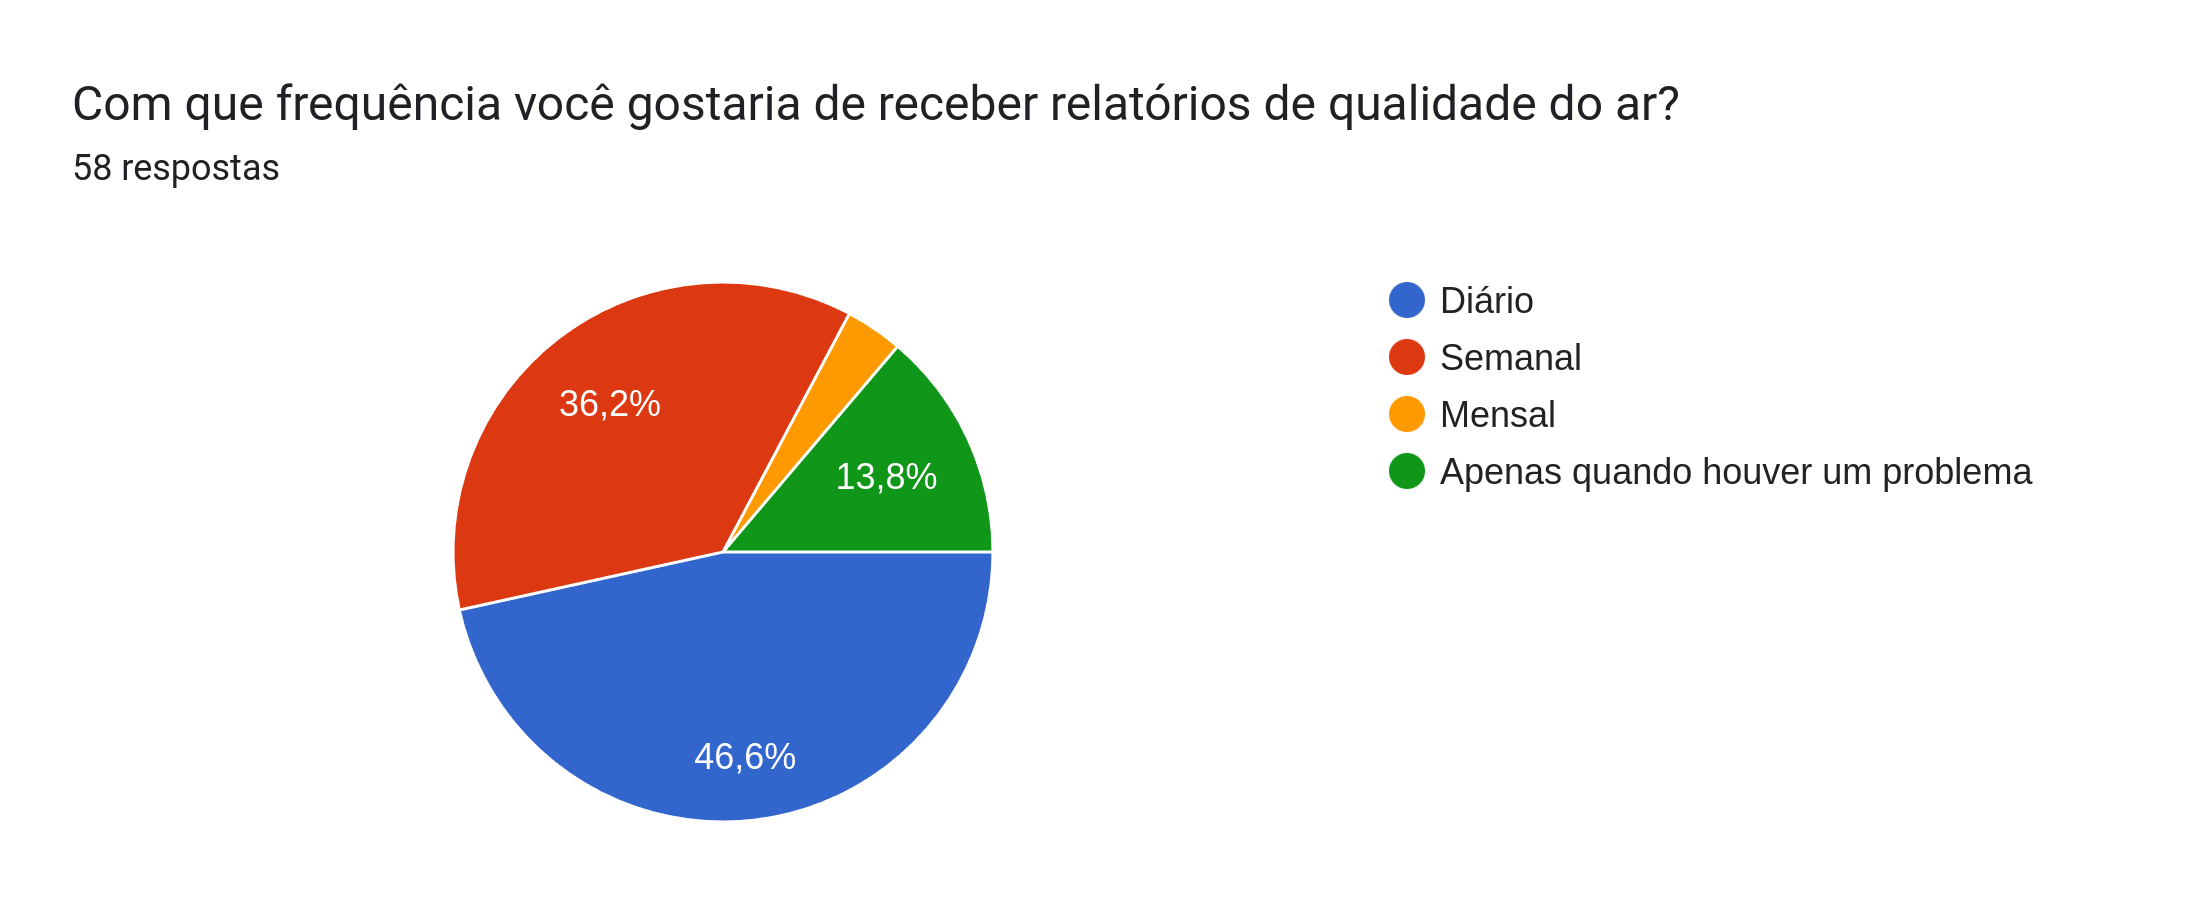
\includegraphics[width=.64\textwidth]{img/questionario/1/graf-info-frequencia.png}
    \caption{Pergunta sobre frequência de coleta de dados e aviso de problema. Fonte: Autor.}\label{grafFrequenciaInfo}
\end{figure}

Para concluir a análise das respostas do primeiro questionário, a pergunta apresentada aos alunos — \textit{``Como você imagina que um dispositivo de medição da contaminação do ar pode melhorar sua qualidade de vida?''} — proporcionou boas motivações. Muitos 
entrevistados mencionaram sintomas respiratórios enfrentados durante períodos de queimadas, ressaltando que um sistema desse tipo seria útil na prevenção dos efeitos nocivos da fumaça para a saúde. O protótipo possui 
relevância informativa, pois permite ao usuário monitorar, em tempo real, as condições ambientais. Contudo, seu papel vai além da mera apresentação de dados, ao fornecer ao dispositivo móvel eventos do ambiente 
acompanhados de descrições detalhadas.

O segundo questionário envolve a execução de tarefas reais com o sistema embarcado. Ao todo, 38 alunos de graduação participaram 
do experimento, com duração média de 30 minutos e grupos formados por duas ou três pessoas. O uso de grupos no teste de usabilidade, e não indivíduos separadamente, é justificado 
pela quantidade grande de participantes e também pela particularidade da tarefa 8, pois sua execução necessita de dois usuários ativos para ocorrer a troca de propriedade. Portanto, 
a Figura \ref{grafAtvResultado} ilustra o resultado geral da execução de atividades descritas na Tabela \ref{tab:cenarios-de-uso}. 

\begin{figure}[ht]
    \centering
    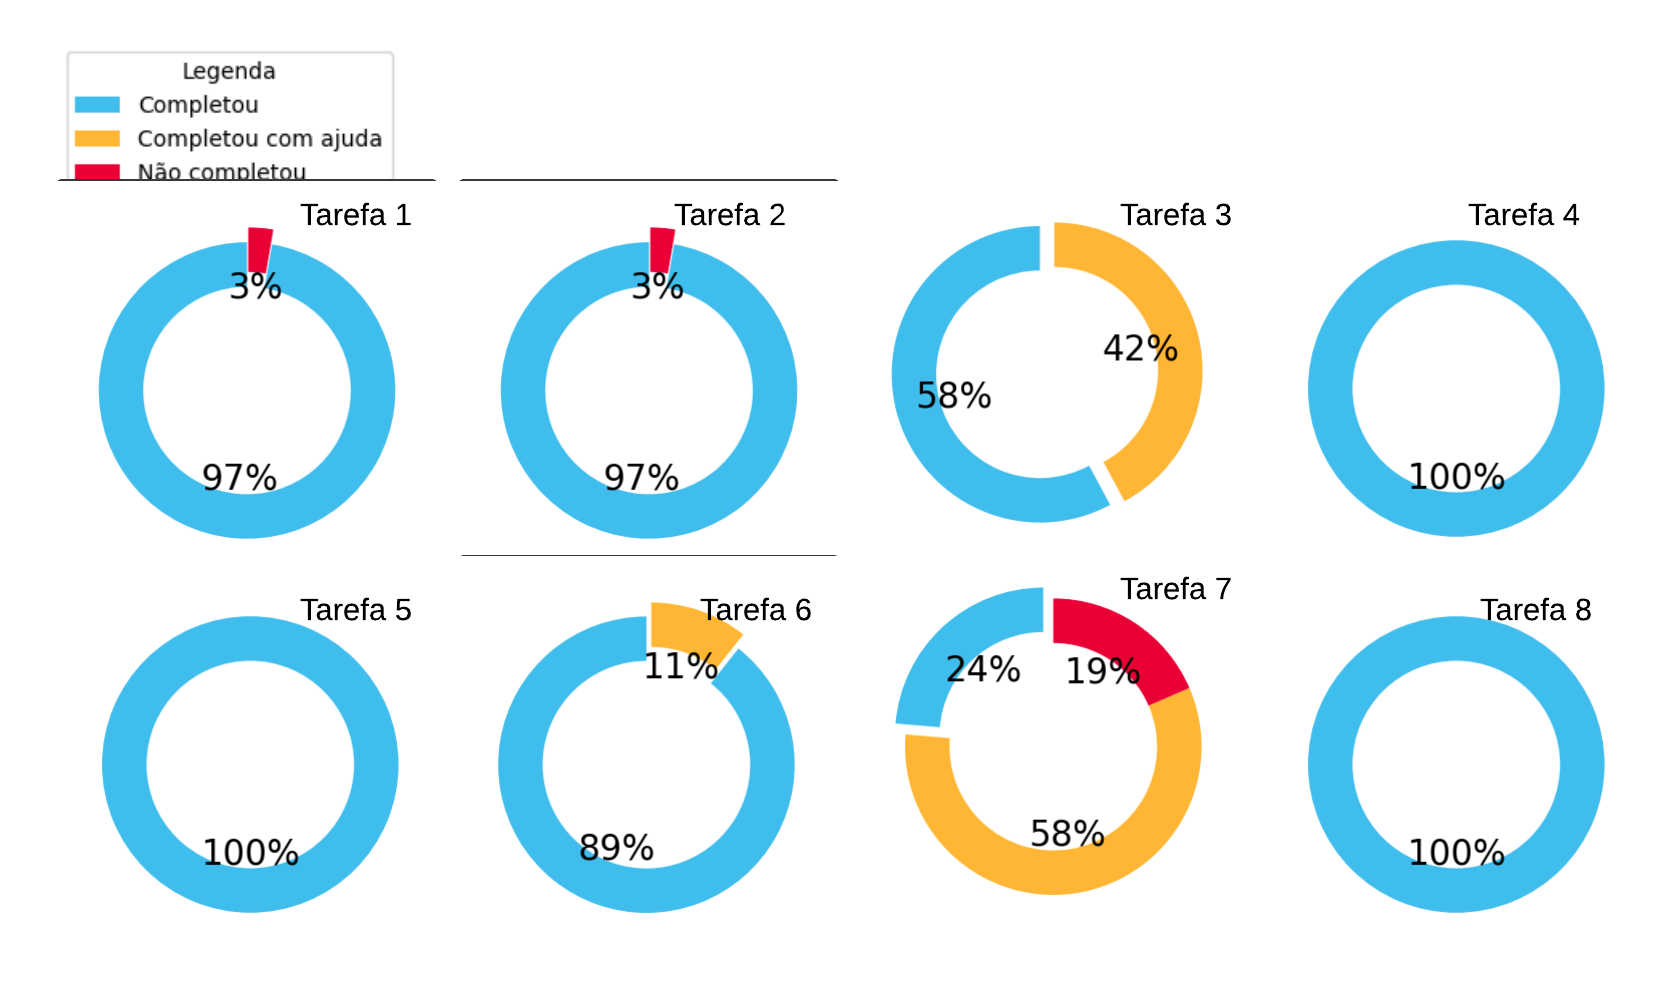
\includegraphics[width=.94\textwidth]{img/questionario/1/graf-atividades-resultado.png}
    \caption{Resultado das atividades. Fonte: Autor.}\label{grafAtvResultado}
\end{figure}

Após a realização do teste, os entrevistados responderam a um segundo questionário, para coletar opiniões sobre o 
sistema de monitoramento. De modo geral, os participantes conseguiram executar a maioria das atividades com sucesso, uma vez que o manual 
da aplicação foi disponibilizado durante a avaliação, permitindo a consulta em caso de dúvidas. Apesar disso, a tarefa 3, cujo propósito é cadastrar o dispositivo na 
rede Wi-Fi, necessitou de ajuda do desenvolvedor em 42\% dos casos, o que evidencia a complexidade da atividade. Essa tarefa é especialmente rica em 
informações técnicas e requer atenção a detalhes específicos, o que pode representar um desafio para usuários sem familiaridade com configuração de redes de internet.

A tarefa 8, referente ao uso do dispositivo com conexão Bluetooth, também apresentou desafios. Durante o experimento, notou-se uma divergência 
no modo de conexão e emparelhamento do celular de alguns alunos, pois o \textit{smarthphone} reconhece o protótipo embarcado na lista de dispositivos e não executa a ação de ``conectar aparelho''. Portanto, para 
esses casos o funcionamento do sistema no modo \textit{online} é a única opção disponível. 

A seguinte pergunta do questionário apresenta a afirmação — \textit{``Eu acho que o sistema BURI é fácil de usar''} — para avaliar a percepção dos participantes sobre a usabilidade 
do sistema. Foi utilizada uma escala de 1 a 5, sendo 5 equivalente à concordância total e 1 à discordância total. Nessa etapa, os participantes atribuíram notas com base em suas experiências 
individuais. O resultado da pesquisa foi positivo, já que a maioria das notas atribuídas foi 4 ou 5 (ausência de escolhas da opção 2), demonstrando que o sistema atende às expectativas do público-alvo.

\begin{figure}[ht]
    \centering
    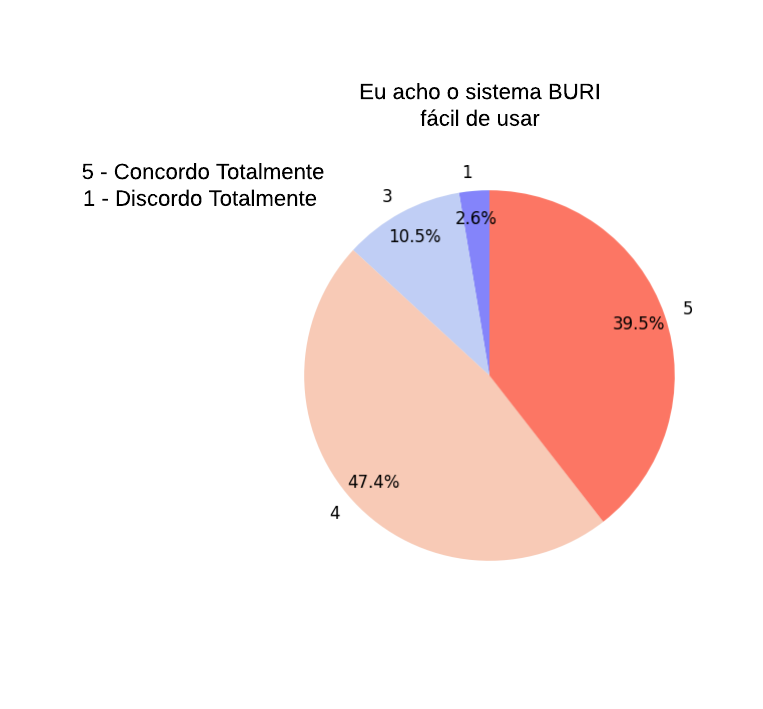
\includegraphics[width=.44\textwidth]{img/questionario/1/graf-sistema-buri-facil-de-usar.png}
    \caption{Resultado da pergunta sobre a facilidade do sistema. Fonte: Autor.}\label{grafBuriFacilDeUsar}
\end{figure}

Sobre a experiência de uso do aplicativo, o projeto recebeu boas avaliações. Entre os pontos positivos, 
usuários destacaram a velocidade de atualização das informações na tela e a troca simplificada do modo de operação no \textit{hardware}, assim como o processo de solicitação de propriedade 
para outro usuário. Os comentários negativos são direcionados ao processo de configuração da rede Wi-Fi e o modo \textit{offline}, pois são atividades 
realizadas com mais dificuldade. Portanto, os comentários obtidos no questionário são fundamentais no processo de melhorias e correções de erros do sistema BURI.


\begin{figure}[ht]
    \centering
    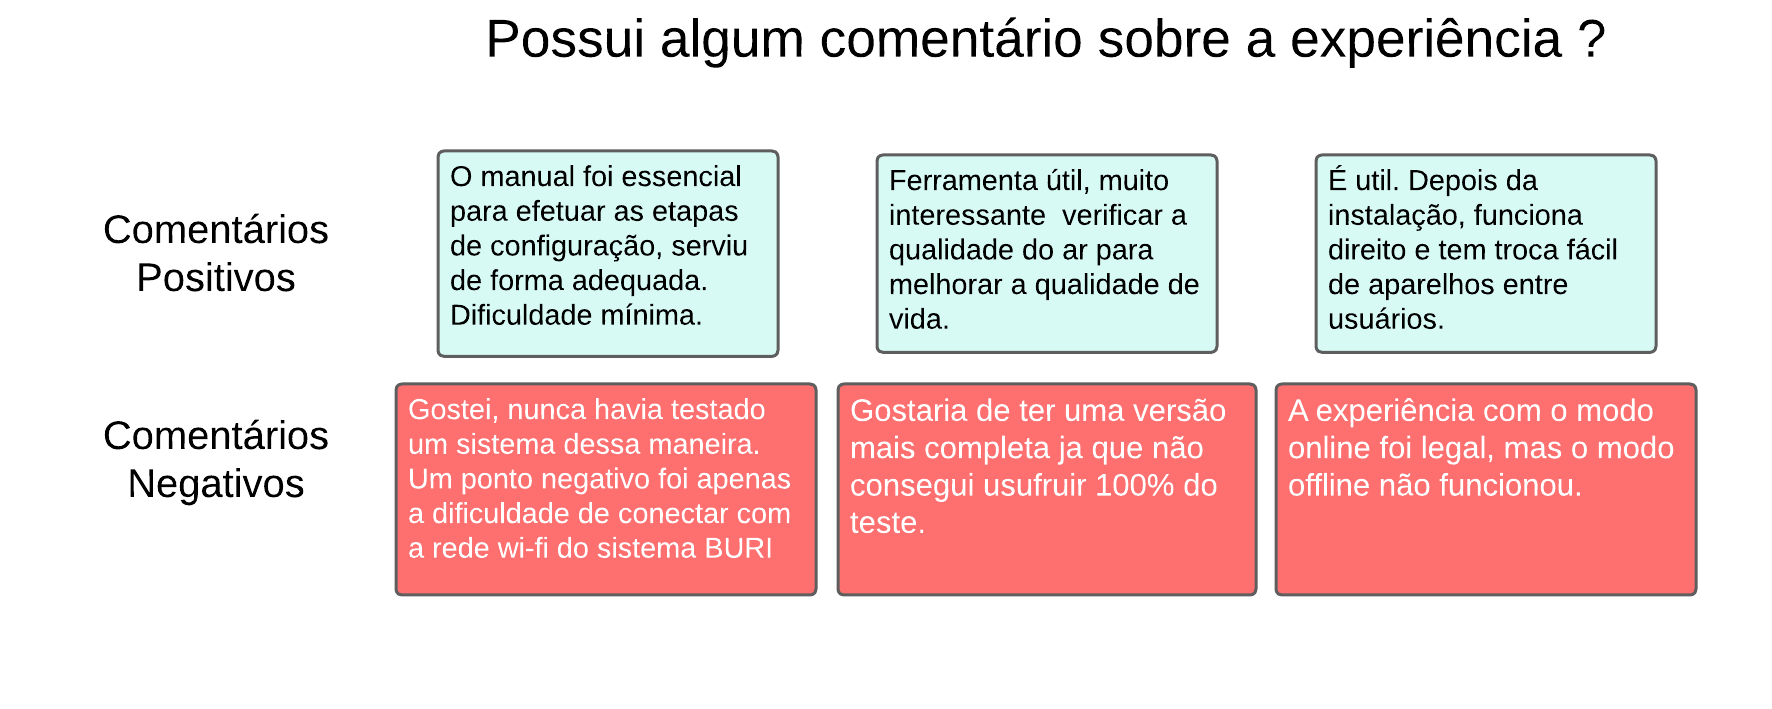
\includegraphics[width=.84\textwidth]{img/questionario/1/relato-comentarios-sistema-buri.png}
    \caption{Comentários positivos e negativos sobre o sistema. Fonte: Autor.}\label{grafComentarios}
\end{figure}

\section{Teste do sistema de alerta}\label{alerta}

\section{Comparação técnica com trabalhos similares}\label{comparacao}

Após a finalização de todas as etapas da metodologia, incluindo a realização de teste de usabilidade com pessoas de diferentes áreas, esta seção trata da análise dos resultados obtidos 
neste trabalho de conclusão de curso em comparação com a literatura atual. A primeira observação de similaridade diz respeito aos sensores utilizados, cuja escolha foi justificada pelos resultados 
apresentados nos respectivos trabalhos de referência. Isso implicou na manutenção dos componentes para o uso no trabalho final. Outra questão relacionada é o uso do microcontrolador ESP32, pois o dispositivo apresenta 
recursos nativamente na placa de desenvolvimento, como Wi-Fi e Bluetooth, ao contrário do Arduino, para o qual seria necessário adquirir os módulos separadamente. O resumo da análise comparativa é apresentado na Tabela \ref{tab:trabalhos-comparativo}.

\begin{table}[htbp]
    \centering
    \caption{Comparativo do sistema BURI com trabalhos de referência. Fonte: Autor.}\label{tab:trabalhos-comparativo}
    \begin{tabular}{p{4cm}|c|c|c|c|c|c}
        \toprule
        \textbf{Trabalho} & \textbf{Dispositivo Físico} & \textbf{Online} & \textbf{Offline} & \textbf{Alerta}  & \textbf{Ação} & \textbf{Código Aberto} \\ 
        \midrule
        \cite{uea-iot-deteccao-incendio} & Sim & Sim & Não & Sim & Sim & Sim \\ \midrule
        \cite{iot-monitoring-on-aws} & Sim & Sim & Não & Sim & Não  & Não \\ \midrule
        \cite{UFAMAirWorld} & Sim & Sim & Não & Sim & Não  & Não \\ \midrule
        \cite{tbRelacionado4NovelEmbeddedSystem} & Sim & Sim & Não & Sim & Não & Não \\ \midrule
        \cite{alexandre-automaccao-formulas-de-leitura-sensor} & Sim & Sim & Sim & Sim & Não & Não \\ \midrule
        Este trabalho & Sim & Sim & Sim & Sim & Não & Sim \\
        \bottomrule
    \end{tabular}
\end{table}

Sobre as diferenças da abordagem atual em relação aos demais trabalhos, destaca-se o foco específico no monóxido de carbono, em detrimento de outros gases 
como gás de cozinha ou fumaça. A justificativa para essa escolha reside no fato de que as fontes de vazamento de CO são variadas e nem sempre acompanhadas de sinais 
olfativos, como incêndios. Por exemplo, deficiência na ventilação de ambientes com combustão incompleta podem liberar quantidades significativas de monóxido de carbono, sem haver percepção imediata do ocupante da residência \cite{carbon-monoxide-poisoning-varon}.

No âmbito da Internet das Coisas, este trabalho se diferencia por oferecer uma solução de monitoramento que prioriza a experiência do usuário. Ao contrário de outras propostas existentes, o sistema BURI foi projetado para ser 
configurado e utilizado por qualquer pessoa, independentemente do perfil técnico. A combinação de um processo de instalação simples e de um manual objetivo torna a solução atrativa para o público, além da proposta de solução 
ser escalável para o uso em diversos ambientes. 